\documentclass[12pt,a4paper]{article}

\usepackage[T2A]{fontenc}
\usepackage[utf8]{inputenc}
\usepackage[russian]{babel}
\usepackage{amsmath}
\usepackage{geometry}
\usepackage{enumitem}
\usepackage{microtype}
\usepackage{graphicx}

\geometry{margin=2.5cm}
\setlist{itemsep=0.3em, topsep=0.5em}
\setlength{\parindent}{0pt}
\setlength{\parskip}{0.6em}

\title{EMTomo: вероятностная томография по временам прихода}
\author{}
\date{}

\begin{document}

\maketitle

\section*{Что мы разрабатываем}

Мы разрабатываем EMTomo --- вероятностный метод сейсмической
томографии по временам прихода, в котором положения источников
рассматриваются как скрытые переменные и оцениваются вместе со скоростной
структурой среды.

Предполагаемое применение --- построение начальных скоростных
моделей для более точных алгоритмов, использующих сейсмограммы целиком,
в частности полноволновой инверсии. Мы не пытаемся заменить эти методы
томографией по первым вступлениям. Наша задача --- получить исходное
приближение без необходимости заранее фиксировать единственную
локализацию каждого события.

В перспективе мы планируем перейти к восстановлению изменений
скоростной структуры во времени. Более дальняя исследовательская цель
--- проверить, несут ли эти изменения дополнительную информацию для
прогнозирования землетрясений. Сейчас основная работа сосредоточена
на 3D-алгоритме EMTomo.

\section*{Основная идея метода}

На вход подаются времена прихода волн от событий и координаты станций.
Неизвестны скоростная модель и положения гипоцентров.

Главная особенность --- работа не только с одной оценкой положения
источника, а с набором возможных положений и их весами. При неточной
скоростной модели локализация события тоже неопределённа. Если сразу
зафиксировать её как точную, ошибка положения может перейти в скоростную
модель. В EMTomo мы стремимся учитывать эту неопределённость
непосредственно при инверсии: несколько гипотез положения одного события
вносят взвешенные вклады в обновление среды.

Алгоритм строится как EM-подобная итерационная схема:

\begin{enumerate}
    \item Расчёт прямой задачи.
    Для текущей скоростной модели методом Fast Marching рассчитываются
    поля времён пробега от станций по всему объёму.

    \item Оценка положений источников.
    Для каждого события рассчитывается пространственное поле невязки.
    Используются разности времён прихода между станциями для одного
    события:
    \[
        (t_i-t_j)_{\text{набл}}
        -
        \bigl(T_i(x)-T_j(x)\bigr)_{\text{расч}}.
    \]
    Это исключает неизвестное время возникновения события. Здесь речь
    именно о межстанционных разностях для одного события, а не
    о межсобытийных double-difference.

    \item Формирование взвешенных гипотез.
    Из поля невязки выбираются пространственно разнесённые кандидаты
    положения гипоцентра, их координаты уточняются внутри ячеек.
    По невязкам рассчитываются нормированные веса. Таким образом,
    неопределённость положения представляется набором взвешенных гипотез.

    \item Обновление скоростной модели.
    Для кандидатов трассируются лучи по градиентам полей времени.
    По длинам лучей в ячейках строится линеаризованная задача на поправки
    к медленности \(s=1/v\). Вклады разных событий и возможных положений
    источников суммируются с соответствующими весами.

    \item Повторение цикла.
    После обновления скоростей пересчитываются поля времён и оценки
    положений источников.
\end{enumerate}

\section*{Параметризация и текущая реализация}

Мы используем ячеечную параметризацию среды, разделяя
расчёт прямой задачи и параметры инверсии:

\begin{itemize}
    \item мелкие расчётные ячейки используются для вычисления
    полей времён пробега, поиска положений источников и трассировки лучей;
    \item крупные скоростные ячейки задают неизвестные параметры
    среды: одна крупная ячейка соответствует одному скоростному
    параметру для выбранного типа волны.
\end{itemize}

Таким образом, значения на мелкой расчётной сетке определяются
крупноячеечной скоростной моделью и не являются дополнительными
независимыми неизвестными. Это позволяет повышать точность прямого
расчёта без пропорционального увеличения числа параметров инверсии.

Для P- и S-волн мы планируем независимые инверсии: модель
\(V_p\) будет восстанавливаться по временам прихода P-волн, а модель
\(V_s\) --- по временам прихода S-волн. Совместная инверсия двух типов
волн с заданной связью между \(V_p\) и \(V_s\) в текущий план не входит.
Основная отладка сейчас ведётся для \(V_p\).

Инверсия выполняется через накопление взвешенных нормальных уравнений.
Межстанционные разности учитываются без явного построения всех пар
строк. Для стабилизации используются:

\begin{itemize}
    \item диагональная регуляризация поправок;
    \item усиленное подавление обновлений в ячейках с низкой
    дифференциальной чувствительностью;
    \item ограничение относительного изменения скорости за итерацию.
\end{itemize}

\section*{Текущий статус}

Реализован вычислительный прототип полного итерационного цикла:

\begin{itemize}
    \item генерация синтетических времён прихода, в том числе с шумом;
    \item расчёт полей времён;
    \item поиск и уточнение гипотез положения источников;
    \item вычисление их весов;
    \item трассировка лучей и перенос чувствительностей на крупные
    скоростные ячейки;
    \item решение обратной задачи и обновление скоростей;
    \item сохранение моделей, невязок и диагностических величин,
    просмотр результатов.
\end{itemize}

Первый тест проведён на синтетическом объёме
\(4{,}5 \times 4{,}5 \times 4{,}5\)~км,
разбитом на \(9 \times 9 \times 9\) скоростных ячеек
со стороной 500~м. Для прямой задачи используются
\(72 \times 72 \times 72\) расчётные ячейки
со стороной 62{,}5~м. Для инверсии \(V_p\) это соответствует
729 неизвестным скоростным параметрам.

Используются 64 станции на верхней поверхности и 250
синтетических событий. Истинная модель содержит плавную центральную
низкоскоростную аномалию до \(8\%\) на фоне
\(V_p=5\)~км/с; инверсия начинается с однородной модели.

В первом тесте оба алгоритма качественно восстанавливают центральную
неоднородность; результат EMTomo визуально находится на уровне TomoDD.
Количественное сравнение метрик пока не проведено. Сейчас мы ищем
скоростную модель реального региона для второго этапа проверки.
Работоспособность на реальных временах прихода пока не проверена.

\section*{Пример работы алгоритма}

На рисунках показан синтетический пример: начальная и истинная модели,
результат EMTomo после 17-й итерации и распределение весов гипотез
положения для одного события. Цветовые шкалы на рисунках заданы
независимо.

\begin{figure}[htbp]
    \centering
    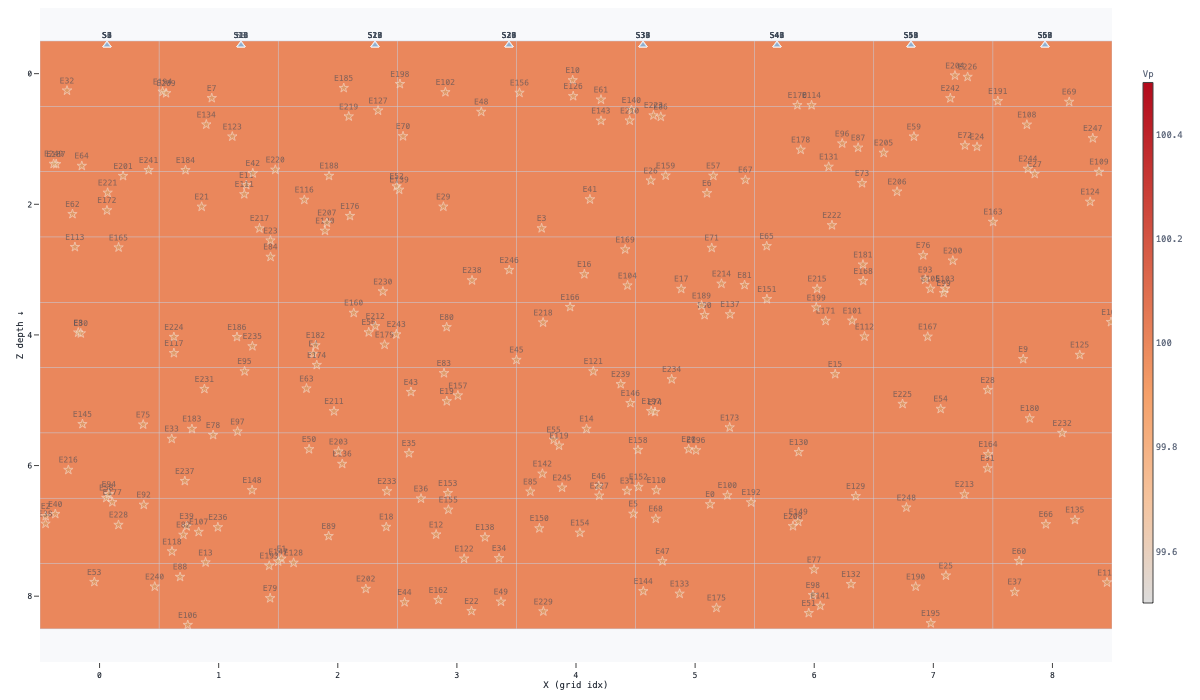
\includegraphics[width=0.49\textwidth]{run_20260903_143109_iter_0_velocity-2.png}\hfill
    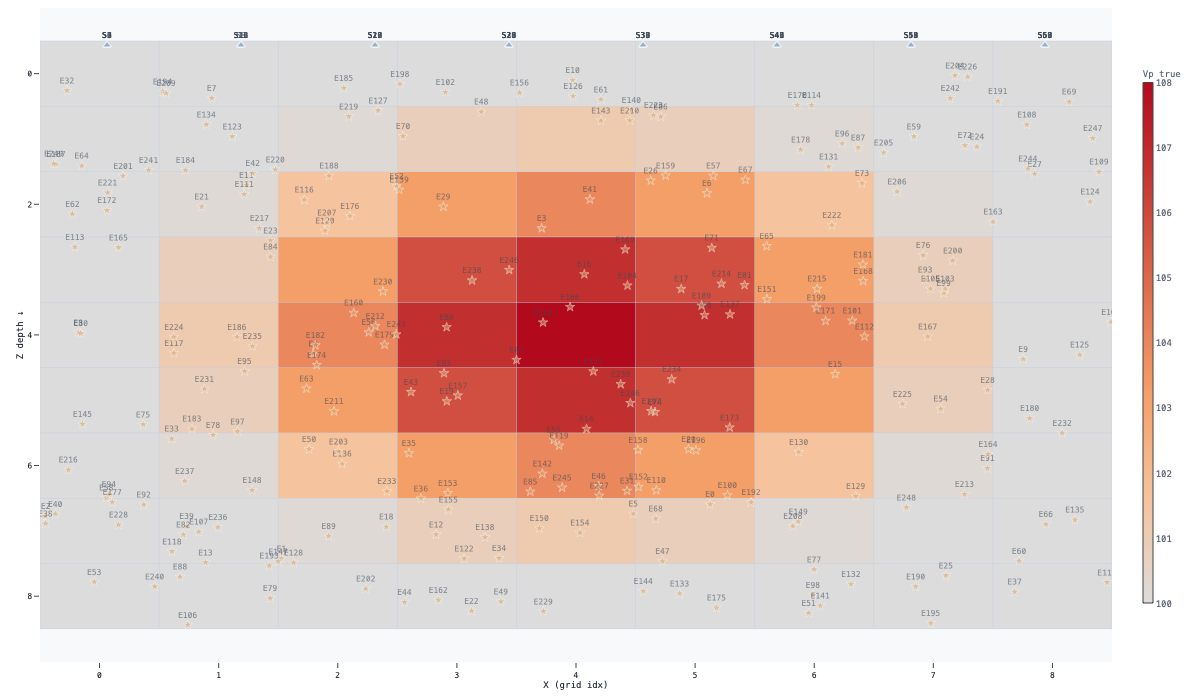
\includegraphics[width=0.49\textwidth]{run_20260903_143109_iter_0_true_model-2.png}
    \caption{Слева --- начальная однородная скоростная модель. Справа ---
    истинная модель с центральной скоростной неоднородностью.}
\end{figure}

\begin{figure}[htbp]
    \centering
    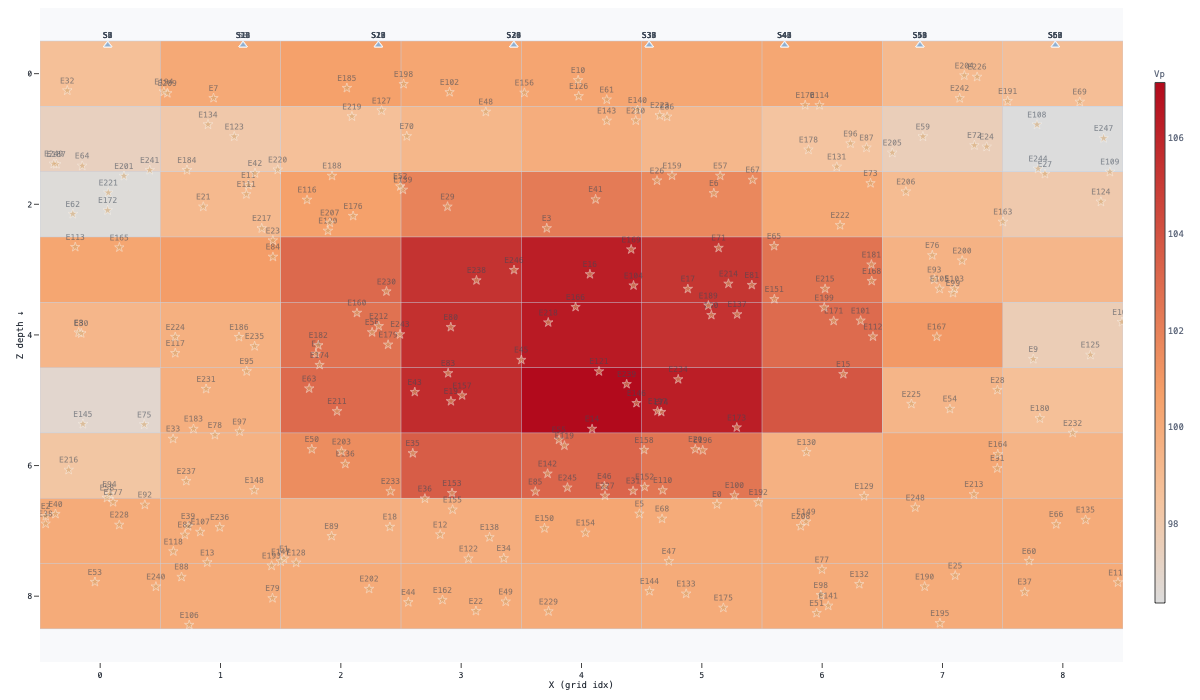
\includegraphics[width=0.92\textwidth]{run_20260903_195317_iter_17_velocity-2.png}
    \caption{Скоростная модель, восстановленная EMTomo после 17-й итерации.
    Центральная неоднородность восстанавливается качественно.}
\end{figure}

\begin{figure}[htbp]
    \centering
    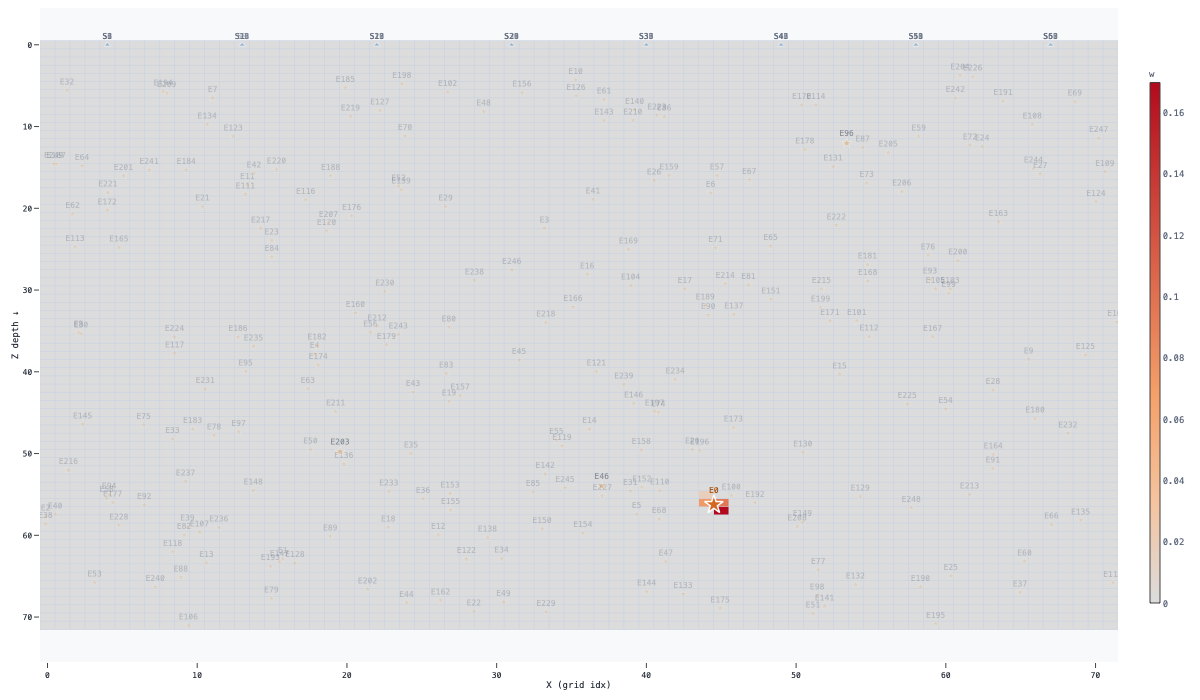
\includegraphics[width=0.92\textwidth]{run_20260903_195317_iter_17_hypo_weights-2.png}
    \caption{Пример распределения весов гипотез положения для одного события.
    Максимальный вес сосредоточен вблизи выбранного положения источника.}
\end{figure}

\clearpage

\section*{План проверки метода}

Проверка включает три этапа.

\begin{enumerate}
    \item Упрощённая синтетическая модель с одной неоднородностью
    в центре объёма.

    Первый тест уже проведён: EMTomo качественно восстанавливает
    центральную неоднородность на уровне TomoDD. Количественное
    сравнение ошибок восстановления скоростей, формы и амплитуды
    аномалии, а также локализации источников ещё не выполнено.

    \item Реальная скоростная модель с синтетическими событиями
    и временами прихода.

    Сейчас мы ищем подходящую скоростную модель реального региона.
    Она будет использоваться как эталон для генерации синтетических
    событий и времён прихода и последующей оценки восстановления.
    Это позволит проверить алгоритм на более сложной структуре
    при известных параметрах синтетического эксперимента.

    \item Полностью реальные времена прихода.

    На этом этапе мы планируем применить EMTomo к наблюдённым временам
    прихода и реальной геометрии сети. Поскольку истинная скоростная
    структура и точные положения источников здесь неизвестны,
    одной невязки будет недостаточно: потребуется оценка устойчивости
    результата и сопоставление с независимыми данными и другими методами.
\end{enumerate}

Количественное сравнение с TomoDD запланировано обязательно,
с LOTOS --- возможно. Мы будем сравнивать не только итоговую невязку, но и
восстановление скоростной структуры, ошибки локализации там, где они
известны, а также устойчивость к стартовой модели и шуму.

Отдельно необходимо проверить именно пользу вероятностной части:
даёт ли учёт нескольких гипотез положения источника преимущество перед
схемой, которая на каждой итерации использует одну фиксированную
локализацию.

\section*{Итого}

Мы разрабатываем EMTomo как вероятностный инструмент восстановления
скоростей и положений источников по временам прихода, прежде всего для
подготовки начальных моделей к более точной инверсии полных сейсмограмм.
Крупные ячейки задают независимые скоростные параметры, а мелкие
используются для расчёта времён пробега. Инверсии для P- и S-волн
планируются независимыми.

Первый синтетический тест показал, что EMTomo качественно
восстанавливает неоднородность на уровне TomoDD; количественное
сравнение метрик ещё не проведено. Сейчас мы ищем эталонную
скоростную модель для второго этапа, после которого планируется
тест на реальных временах прихода. Преимущество вероятностного
подхода и пригодность результатов как начальных моделей для
полноволновой инверсии пока не установлены.

\end{document}
